%!TEX root = ../document.tex

\section{Point of View} \label{sec:POINT_OF_VIEW}

A point of view (POV) consists of three parts: a concrete specification of the user we are designing for, his/her needs that we are trying to satisfy with our solutions and finally a [surprising] insight that was derived from the understanding and observation phase. We present all of these in this section.

We derive a "How might we..." question from our POV and this question in our ideation phase. This description presents the final Persona and her needs. Throughout the course the persona was changed slightly as we discovered new needs and reevaluated their importance for our persona. 

\subsection{Persona}
\label{subsec:persona}

Our Persona is Amber, she is 31 years old and works as a Software Developer for roughly 6 years at a big company that is using HANA as a database for its application. She works in team of 10 developers. She develops applications that work on big data sets and are performance critical. Her focus is more on the backend side. She is not a database expert but knows how to write SQL queries. However, she is not able to predict the impact of certain changes in query formulation on performance just by looking at the statement. She works in her favorite development environment studio, which is eclipse. She uses the HANA Eclipse Studio if she wants to look at the content or schema of the database.

Amber enjoys coding a lot. It is the favorite part of her work. She is also very enthusiastic and wants to get feature completed as fast as possible. She uses a lot of different tools that help her to simplify reoccurring tasks and boosts her productivity.

Throughout her work day Amber is interrupted a lot. We refer to these interrupts as context switches that pull her out of her workflow. These might be small context switches, like changing from the editor to the browser and looking something up online. Large context switches such as having to write an email or getting interrupted physically by someone else also disrupt her flow.

\begin{figure}
    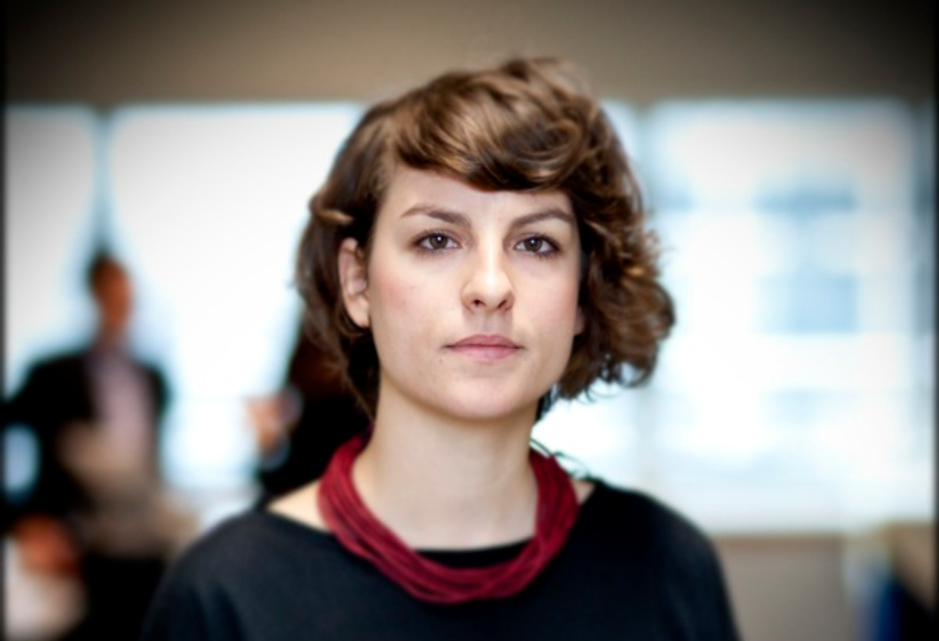
\includegraphics[width=\linewidth]{images/amber}
    \caption{Our persona Amber.}
    % #selfrespect
    \label{fig:amber}
\end{figure}

\subsection{Needs}
Amber's needs are manyfold. The most important ones are:

\begin{itemize}
	\item She wants to get work done as efficiently as possible
	\item Since her applications are performance critical she needs to evaluate performance of her code on real customer data.
	\item Amber is not an SQL expert. She needs a way to explore and learn which parts of a query perform well and which parts are bottlenecks.
	\item She wants her productivity tools to be integrated into her IDE so that she does not have to switch contexts
	\item The number of context switches in general needs to be decreased
\end{itemize}

The importance of the last point was down-weighted throughout the course of the seminar as we narrowed down the interruptions that we want to tackle. We discovered that although big context switches like answering emails etc. lead to a longer disruption, they occur way less frequent than small context switches between applications. Accumulated, tackling small context switches may lead to a big increase in efficiency which is why we focused on that.  

\subsection{Insight}

During our observation we saw how our persona interacted when she had to understand SQL queries written in code. She copied the query into the HANA Studio, had to escape all quotes. This is the first context switch. Most queries contain parameters that are bound during runtime. In order to execute the query in the Studio Amber looks up appropriate values in the schema. This is the second context switch. If the executed query does not answer as expected she has to switch back and forth in the Studio between edit-mode and result-view mode. There is no way to see the impact of changes in the query on the result in the same window. This are a number of additional context switches. If the query finally behaves as wanted, Amber has to copy it back into code and replace the concrete values by variables again.  

We consider this interaction as a workaround and take it as a foundation for our point of view as it emphasizes the most important need: Predicting the impact of queries on the underlying data. We combined our Persona and her need with one of the insights we gathered during our interviews, namely that \textit{Code needs data context} (cf. Section \ref{sec:UNDERSTAND}).


\subsection{POV Statement}

\begin{description}
	\item [User] Amber, a productivity junkie, working with HANA on performance critical big data business applications.
	\item [Need] Amber need to predict the performance and logical impact of her code on the underlying data sets without switching to another application.
	\item [Insight] Code needs data context.
\end{description}

From that we derived the following "How might we question...":

\subsection{How Might We...}

\begin{quote}
\emph{"How might we help Amber to predict the impact of her code on the real customer data right in her development environment?"}
\end{quote}